\tikzsetnextfilename{circular_channel}

% Note how the size of all node text has been increased
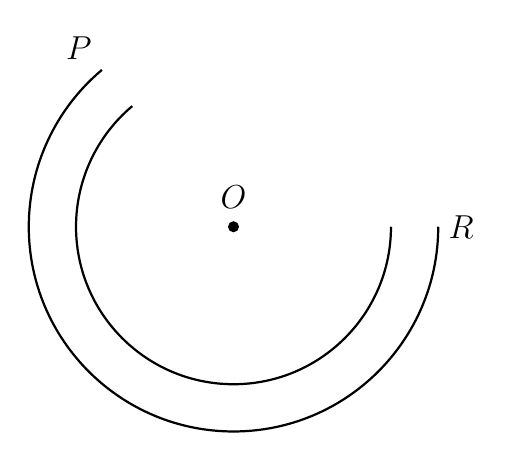
\begin{tikzpicture}[every node/.append style={font=\large}]

    \def\ri{2}
    \def\ro{\ri * 1.3}      % Set outer radius as 30% larger than the inner radius

    \fill
        (0,0) circle (2pt) node[anchor=south, yshift=3pt] {$O$}
    ;

    \draw[thick]
        (\ri,0) arc (0:-230:\ri)        % Start arc on x-axis and the swing through to -230 degrees with radius \ri
        (\ro,0) node[anchor=west] {$R$} arc (0:-230:\ro) node[anchor=south east] {$P$}
    ;

\end{tikzpicture}
